\section{Tokenstream}\label{sec:yourmethod}

\todo{pptranducer} 

\subsection{Overview}

The method that we propose can be viewed as a batch processing system consisting
of four components (Figure \ref{fig:methodoverview}):

\begin{figure}[tb]\centering
	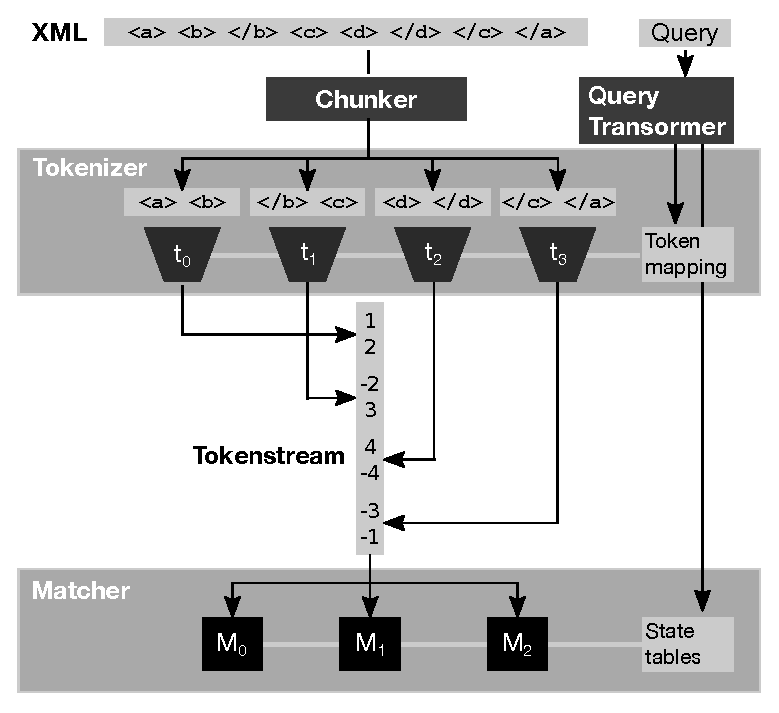
\includegraphics[width=.5\textwidth]{img/methodoverview.eps}
  \caption{Batch view of the system.\label{fig:methodoverview}}
\end{figure}

\begin{enumerate}
\item The query transformer, \item the chunker, \item the tokenizer, and \item the matcher.
\end{enumerate}

First, a \emph{Query Transformer} analyzes the query and produces a \emph{token
mapping} and a state table describing a push-down automaton for each XPath
expression in the query.

The \emph{chunker} splits the XML streams into chunks of approximately equal
size. Each opening or closing tag (e.g. \verb;<a>;, or \verb;</a>;) is fully
contained in a chunk, however the structure of the XML data contained in the
individual chunks can be arbitrary.

The \emph{tokenizer} then compresses each XML chunk into a tokenstream chunk,
using the token mapping generated by the query transformer to map tag names to
token ids. Connected together, these tokenstream chunk form the tokenstream. In
the \emph{matcher}, the push-down automatons are run in parallel over the
entire tokenstream to identify matching nodes.

The aim of our method is to reduce memory traffic in the matching phase, as the
tokenstream takes up less memory than the original XML stream. Workloads are
divided differently in the tokenizer and in the matcher. Our method is
successful if we achieve \emph{strong scaling} for the tokenizer and \emph{weak
scaling} for the matcher.

\subsection{Query Transformer}

The query transformer takes as input an XPath query which takes the form of a
text file containing one or more XPath expression. The query transformer outputs
two text files: a token mapping and a file containing the state tables of
the push-down transducers, one for each path expression in the input file.

A token mapping is simply a list that contains all tag names appearing in any
of the path expressions. The line number corresponds to the token id for the
tag name on that particular line. These token numbers serve as input alhpabet
of the push-down automatons.

The push-down automatons are generated using the methods presented in \todo{xml
processing paper}: Each path expression is turned into an query tree. However,
as opposed to \todo{same paper as above}, we build a query tree for each
individual path expression. This query tree is in turn used to generate a
non-deterministic automaton which is then transformed into a deterministic
automaton using the standard power set method described in \todo{ulman
reference}.

\subsection{Chunker}

The chunker splits the input XML file into chunks of approximately equal size.
The minimum size of a chunk is determined by dividing the size of the XML
document by the number of available threads in the tokenizer. The first chunk
starts the beginning of the XML stream. The start of the following chunk is
determined by adding the minimum chunk size to the current position and
searching for the next less-than-sign ('\texttt{<}')–these offsets accumulate over
all chunks, rendering the last chunk smaller than the minimum chunk size, but we
assume that the effects of this are negligible for our considerations.

Similar to \todo{transducer} we ignore \texttt{CDATA}-sections and comments for
simplicity. The authors of \todo{transducer} suggest extending the transducer to
accommodate the possibility that a chunk starts within a comment or a
\texttt{CDATA}-section. Similarly, in our case, the tokenizer could just output
tokens for the start and end of comments and \texttt{CDATA}-sections.

\subsection{Tokenizer and Tokenstream}

The tokenizer maps tag names onto corresponding token nubmers according to the
token mapping generated by the query transformer: A top-down parser parses the
XML and whenever an opening or closing tag is found, the tag name is compared
with a list of known tag names from the token mapping. For closing tags, the
token number is negated. All unknown opening (closing) tags, i.e. tag names that
do not appear in any of the path expressions, are mapped onto the token number
$n+1$ ($-(n+1)$).

For example, consider an XML chunk \verb;<a><c></c></a>; and a token mapping
containing only the tag names \verb;a; and \verb;b; in this order. The
aforementioned XML chunk would be translated into the token stream $1, 3, -3,
-1$.

In our implementation, the token numbers are encoded as 16-bit wide signed
integers. This seemed to be reasonable trade-off between the number of different
tag names ($2^{15}-2$) that can be represented and encoding size. Note that the
token size can in principle also be decided dynamically based on the size of the
token mapping.

Similarly to the tokenstream, each thread also outputs a chunk of the
\emph{offset stream} which contains the byte offset for each tag. \todo{this
could be compressed}

As we implemented our method on a Xeon Phi \todo{reference to spec} which is a
shared memory machine, we employed the fork-join paradigm offered by OpenMP
\todo{reference} to manage thread allocation and synchronization. Each XML chunk
can be tokenized independently of all the others, and thus there is no need for
further synchronization between the threads when the threads are running.

\subsection{Matcher}

The matcher runs each push down automaton in a separate thread. Hence, the
number of threads is equal to the number of path expressions in the original
XPath query. As soon as a push-down automaton transitions into an accepting
state, the offset of the matching token in the token stream is written into an
output stream. Hence, the character offset of a matching tag in the original
XML, can be found by fetching the value in the offset stream at the position
found in the output stream.

For simplicity, our implementation only outputs the character offset of the
opening and closing tags which belong to the matching node.

%Now comes the ``beef'' of the report, where you explain what you
%did. Again, organize it in paragraphs with titles. As in every section
%you start with a very brief overview of the section.

%In this section, structure is very important so one can follow the technical content.

%Mention and cite any external resources that you used including libraries or other code.
